\chapter{Evaluation}
\label{cha:evaluation}
This section will now present an evaluation of the authentication and authorization framework in regards to the security requirements. It must be here understood that for a real system to be said \textit{secure}, both the protocols it uses and its implementation must be secure. Code injection for example (SQL, xss), is in any circumstances provoked by a lack in the implementation. Here, the focus will be only put on the protocols. The implementation will be discussed in the next chapter (see Chapter \ref{cha:implementation}).

\section{The verification method}
When evaluating protocols and how secure they are, two main approaches are to be considered. The former tries, from a mathematical background (assumptions and logic rules, for instance) to demonstrate theoretically that the protocol is correct. The latter tries to break the protocol by finding flaws in the design.

The BAN logic is one of the most famous logic used to demonstrate the correctness of a protocol. Its founders,  Burrows, Abadi and Needham determined ways to define objects and protocol tasks. With the assumption that encryption cannot be broken, security properties can then be deduced from the predefined objects and tasks. Even if it has been proven that the BAN logic couldn't find every flaw due to its design, it is still used for security evaluation.

There are also several techniques for finding flaws in a protocol design. One of the field that has been researched the most is the use of state-machines. One could define the protocol logic and some critical security goals that must be met, assume that those goals are not met, and with the help of state machines, finding all the states from which this insecure situation could have been reached. Recursively, security flaws are found. Luckily, there exist automated tool that find security breaches. The Automated Validation of Internet Security Protocols and Applications (AVISPA) tool uses for instance logic to analyze security properties of Internet protocols. The fist step is to describe logically the protocol (who are the actors, what messages they send or receive, etc); the second is to perform automated analysis based on 3 different techniques above discussed: On the Fly Model Checker (OFMC), constraint  logic-based Attack Searcher (AtSe), and SAT-based Model Checker (SATMC).

Both approaches are interesting, but finding a logic that fits a distributed system like the \emph{device cloud} and that could detect every possible flaw mightbe difficult. Hence, AVISPA has been used. 

The next sections describe how the protocol logic has been modeled and present the result of the AVISPA analysis.

\section{The protocol logic}
As seen in Fig. \ref{fig:example}, the authentication framework can be divided into two independent parts: the delegated authentication process (\ref{fig:example_a}) and the direct authentication, which is required when accessing protected resources like consumer profiles or redirectURIs (\ref{fig:example_b}). Thus, the logic will be separated into two different protocols.

To model the logic, AVISPA uses the description language called High Level Protocol Specification Language for industrial security-sensitive protocols (HSPSL) whose goal is to provide a human readable and powerful language to specify the security protocols. The specifications is done by defining roles: one role per actor in the protocol, one recommended role session that binds several actors in one session, and one required role Environment that defines sessions with the appropriate elements. Besides, the knowledge of an intruder can be specified for a better attack analysis.

HSPSL encompasses several types to be used. Agents, for example, are entities playing roles. HSPSL defines also channels (communication between agents), symmetric\_key, public\_key (private-public key infrastructure), text(used as nonce) or message that allows for a detailed description of any protocol. It doesn't provide support for SSL, but with a combination of symmetric keys for encryption and public-private keys for certificate-authentication and signature, it can be simulated. The logic used for the evaluation of the authentication framework can be found in appendix \ref{appendix:hlpls}.

\subsection{Direct Authentication}

This section aims at proving that the direct authentication of the framework is safe. In addition, it also aims at proving that after having authenticated, a protected resource can be securely requested and transmitted. With the described logic, the protocol of this direct authentication and the request of the protected resource is given in Fig. \ref{fig:AVIVA_direct_auth}.

\begin{figure}[!htbp]
	\centering
	\caption{Direct Authentication with AVIVA (HSPSL logic)}
	\label{fig:AVIVA_direct_auth}
	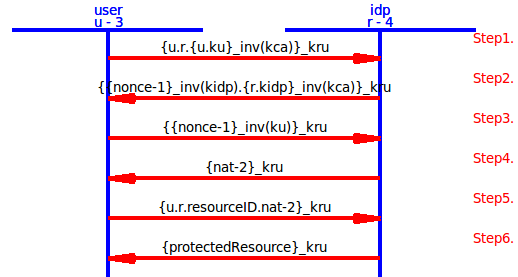
\includegraphics[width=1\textwidth]{images/prot_eva_2.png}
\end{figure}

As said before, all communication channels are encrypted with a symmetric key to imitate SSL ($\{encryptedMessage\}\_key$). Besides, all entities have a public key $ka$ where $a$ is the entity name. The private keys are obtained from the public keys with the $inv$ operator: $inv : ka \rightarrow inv(ka)$.

The process follows the next steps:
\begin{description}
	\item[Step 1] The user $ u $ sends an authentication request to the IdP $ idp $, with its id, the id of the IdP, and its certificate signed by the CA $ \{u.ku\}\_inv(kca) $.
	\item[Step 2] This step and the next ones imitate the SSL certificate authentication. The user has sent a valid certificate in step 1, but it must still prove that it owns the corresponding private key. At the same time, to perform mutual authentication, the server needs to send its certificate and a signed message.
	 \\ Therefore, the IdP sends a generated nonce signed with its private $ \{nonce-1\}\_inv(kidp) $ and its certificate $ \{r.kidp\}\_inv(kca) $ . It expects in return the same nonce signed with the private key corresponding to the certificate given in Step 1.
	\item[Step 3] The user decrypt the nonce $ nonce-1 $ with the public key of the server and sends it back, signed with its private key.
	\item[Step 4] The Server authenticates the user and opens a session. The sessionID is returned: $ nat-2 $.
	\item[Step 5] The user requests a protected resource of id $ resourceID $ and attaches its sessionID $ nat-2 $.  
	\item[Step 6] The protected resource is returned back by the IdP.
\end{description}

In the six different steps, only one assumption is made. Indeed, the entities communicate through encrypted channel (here with a symmetric key) and they trust another entity only if the certificate of this entity has been signed by the CA. In other words, it is assumed that all entities trust the Root Domain (as the Certificate Authority).

The steps observed with AVISPA have been created during a session with a valid End-User and a valid IdP. To check the resilience of the algorithm, 2 more sessions are defined: one with an intruder instead of an End-User and another one with an intruder instead of the IdP. The intruder knows at the beginning the legitimate participants and their public keys. The authentication of the End-User to the IdP as well as the secrecy of the protected resource have been set as critical security goals.

Then, the three verification method previously discussed have been used to detect flaws in the protocol. The result of this analysis is shown in Tab. \ref{tab:result_1}. A more detailed output is given in appendix \ref{appendix:AVISPA_results}.

\begin{table}[!hpbt]
	\centering
	\caption{Result summary of the direct authentication evaluation}
	\label{tab:result_1}
	\begin{tabular}{|c|c|}
		\hline Methods &  Result\\ 
		\hline OFMC & SAFE \\ 
		\hline CL-AtSe & SAFE \\ 
		\hline SATMC & SAFE \\ 
		\hline 
	\end{tabular} 
\end{table}

Every method leads to the same conclusion: the direct authentication seems to be safe. This result was expected, because the direct authentication relies in the framework on SSL certificate authentication, which is supposed to be one of the most resilient way of performing authentication. 

Moreover, a protected resource can be transmitted to an after a direct authentication without being compromised during the transfer. This resource is also accessible only by authenticated users.

When analyzing the process, the data privacy is solely ensured by the symmetric\_key encryption ($ \{protectedResource\}\_kru $); in the case of the \emph{device cloud}, the SSL protocol. But this encryption exists whether the authentication process is direct or delegated, since it is a prerequisite of the framework. Hence, it is already possible to affirm that the methods Get URI Protocol and get Consumer Profile can be performed in a secure way, if the request is authenticated.

\subsection{Delegated authentication logic}
With the described logic, the protocol of the delegated authentication is pictured in Fig. \ref{fig:AVIVA_delegated_auth}. Again, all channels are encrypted with symmetric keys and all entities have a public/private key pair.

The delegated authentication corresponds to the following steps:
\begin{description}
	\item[Step 1] the user sends a message to a client: $\{u.nat\}$, with its id $u$ and a  request that requires authentication (here a dummy message $nat$).
	\item[Step 2] the client $c$ redirects the user to its IdP $r$. It adds along security information (nonce for example), a return address (redirectURI) and the ids of all the participants: $\{u.c.r.redirectionURI.nonce\} $. 
	\\This step could theoretically be preceded by the client retrieving the IdP protocolURI. However, since it has been proved that the GetProtoolURI was secured after a direct authentication, this step has been omitted and it has been assumed that the client knows the IdP.
	\item[Step 3] The user transmits the message, and add its certificate signed by the CA: $ \{u.ku\}\_inv(kca) $.
	\item[Step 4-5] Those steps imitate SSL certificate authentication. The user has proved that it had a valid certificate, but it needs to prove that it has the private key corresponding to the certificate. It also need to trust the IdP, i.e. that the IdP is able to sign with its private key. This is the exact same behavior as explained in the direct authentication process.
	\item[Step 6-7] The IdP redirects the user to the client with a signed token $ \{u.r.c.nonce\}\_inv(kca) $ as proof of the user's validity (here, the IdP has been initialized as the root domain, it has thus the CA public key $ kca $). The IdP sends along its certificate signed by the CA so that the client can decrypt the signed token and verify the IdP's validity at the same time. \\
	Again, GetProtoolURI could have been used by the IdP to retrieve the client's valid protocolURI. Instead, it has been put as a-priori knowledge of the IdP.
\end{description}

Again, one assumption made here is that every entity trusts the Root Domain as the Certificate Authority. The other assumption, as explained in Steps 2 and 6, is that the ProtocolUris of the different Operators (as Client or IdPs) were a a-priori knowledge. In a real case, a participant would instead authenticate to the Root Domain and request this ProtocolUri, which has been proved secure in the last section. But this presupposes that every Operators knows how to contact the Root Domain. 

\begin{figure}[!htbp]
	\centering
	\caption{Delegated Authentication with AVIVA (HSPSL logic)}
	\label{fig:AVIVA_delegated_auth}
	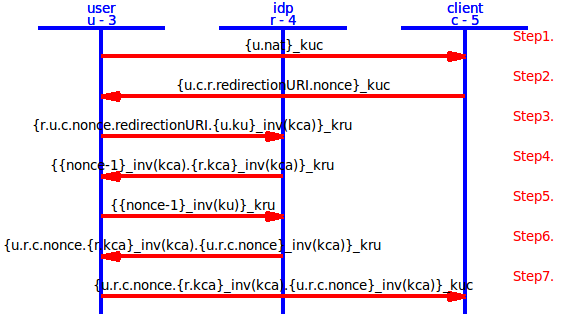
\includegraphics[width=1\textwidth]{images/prot_eva.png}
\end{figure}

The protocol observed in Fig. \ref{fig:AVIVA_delegated_auth} resulted from a session with a valid IdP, a valid End-User and a valid Client. For the evaluation, 4 sessions have been created simultaneously, with respectively no intruder, an intruder as IdP, one as End-User and one as Client. Every time, the intruder's knowledge has been limited to the participants, their public keys and the redirectionURI of the valid Client. It has also been assumed that the intruder could establish a SSL communication any other actor (several symmetric keys have been added to the intruder's knowledge), which basically means that the intruder can establish a SSL secured connection with any valid entity. Of course, this shouldn't be allowed if the certificates are verified with the CA's signature.

The authentication of the end-users to the IdPs (with certificate) and to the clients (with the signed token) are also set as the two critical security goals of the protocol.

The summary of the results is given in Tab. \ref{tab:result_2}. The details can be found in Appendix \ref{appendix:AVISPA_results}.

\begin{table}[!t]
		\centering
		\caption{Result summary of the delegated authentication evaluation}
		\label{tab:result_2}
		\begin{tabular}{|c|c|}
			\hline Methods &  Result\\ 
			\hline OFMC & SAFE \\ 
			\hline CL-AtSe & SAFE \\ 
			\hline SATMC & SAFE \\ 
			\hline 
		\end{tabular} 
\end{table}


As expected, the protocol is declared safe. However, it must be understood that not detecting any flaws in not equivalent to not having any. Hence, so long as no flaws are found by any other means, the framework proposed here can be deemed as secure.


%The End-User HSPSL specification is shown here. The lines beginning with \textbf{\%} are comments.



